\section{x86}

\subsection{\NonOptimizing MSVC}

\RU{Итак, компилируем:}\EN{Let's compile:}

\lstinputlisting{patterns/10_strlen/10_1_msvc_\LANG.asm}

\index{x86!\Instructions!MOVSX}
\index{x86!\Instructions!TEST}
\RU{Здесь две новых инструкции: \MOVSX и \TEST.}
\EN{Two new instructions here: \MOVSX and \TEST.}

\label{MOVSX}
\RU{О первой: \MOVSX предназначен для того чтобы взять байт из какого-либо места в памяти и положить его, 
в нашем случае, в регистр \EDX. 
Но регистр \EDX ~--- 32-битный. \MOVSX означает \IT{MOV with Sign-Extent}. 
Оставшиеся биты с 8-го по 31-й \MOVSX сделает единицей, если исходный байт в памяти имеет знак \IT{минус}, 
или заполнит нулями, если знак \IT{плюс}.}
\EN{About first: \MOVSX is intended to take byte from a point in memory and store value in a 32-bit register. 
\MOVSX meaning \IT{MOV with Sign-Extent}. 
Rest bits starting at 8th till 31th \MOVSX will set to $1$ if source byte in memory has \IT{minus} 
sign or to 0 if \IT{plus}.}

\RU{И вот зачем все это.}\EN{And here is why all this.}

\RU{По стандарту \CCpp, тип \Tchar ~--- знаковый. Если у нас есть две переменные, одна \Tchar, а другая \Tint 
(\Tint тоже знаковый), и если в первой переменной лежит $-2$ (что кодируется как \TT{0xFE}) и мы просто 
переложим это в \Tint, 
то там будет \TT{0x000000FE}, а это, с точки зрения \Tint, даже знакового, будет $254$, но никак не $-2$. 
$-2$ в переменной \Tint кодируется как \TT{0xFFFFFFFE}. И для того чтобы значение \TT{0xFE} из переменной типа 
\Tchar переложить 
в знаковый \Tint с сохранением всего, нужно узнать его знак, и затем заполнить остальные биты. 
Это делает \MOVSX.}
\EN{\CCpp standard defines \Tchar type as signed. If we have two values, one is \Tchar 
and another is \Tint, (\Tint is signed too), and if first value contain $-2$ (it is coded as \TT{0xFE}) 
and we just copying this byte into \Tint container, there will be \TT{0x000000FE}, and this, 
from the point of signed \Tint view is $254$, but not $-2$. In signed int, $-2$ is coded as \TT{0xFFFFFFFE}. 
So if we need to transfer \TT{0xFE} value from variable of \Tchar type to \Tint, 
we need to identify its sign and extend it. That is what \MOVSX does.}

\RU{См. также об этом раздел}
\EN{See also in section} ``\IT{\SignedNumbersSectionName}''~(\ref{sec:signednumbers}).

\RU{Хотя, конкретно здесь, компилятору врядли была особая надобность хранить значение \Tchar в регистре \EDX 
а не его восьмибитной части, скажем, \DL. Но получилось, как получилось: должно быть, 
\gls{register allocator} компилятора сработал именно так.}
\EN{I'm not sure if the compiler needs to store \Tchar variable in the \EDX, it could take 8-bit register part 
(let's say \DL). Apparently, compiler's \gls{register allocator} works like that.}

\index{ARM!\Instructions!TEST}
\RU{Позже выполняется \TT{TEST EDX, EDX}. 
Об инструкции \TEST читайте в разделе о битовых полях~(\ref{sec:bitfields}).
Но конкретно здесь, эта инструкция просто проверяет состояние регистра \EDX на $0$.}
\EN{Then we see \TT{TEST EDX, EDX}. 
About \TEST instruction, read more in section about bit fields~(\ref{sec:bitfields}).
But here, this instruction just checking value in the \EDX, if it is equals to $0$.}

\subsection{\NonOptimizing GCC}

\RU{Попробуем}\EN{Let's try} GCC 4.4.1:

\lstinputlisting{patterns/10_strlen/10_3_gcc.asm}

\label{movzx}
\index{x86!\Instructions!MOVZX}
\RU{Результат очень похож на MSVC, вот только здесь используется \MOVZX а не \MOVSX. 
\MOVZX означает \IT{MOV with Zero-Extent}. Эта инструкция перекладывает какое-либо значение 
в регистр и остальные биты выставляет в $0$.
Фактически, преимущество этой инструкции только в том, что она позволяет 
заменить две инструкции сразу: \TT{xor eax, eax / mov al, [...]}.}
\EN{The result almost the same as MSVC did, but here we see \MOVZX instead of \MOVSX. 
\MOVZX means \IT{MOV with Zero-Extent}. 
This instruction copies 8-bit or 16-bit value into 32-bit register and sets the rest bits to $0$. 
In fact, this instruction is convenient only since it enable us to replace two instructions at once: 
\TT{xor eax, eax / mov al, [...]}.}

\RU{С другой стороны, нам очевидно, что здесь можно было бы написать вот так: 
\TT{mov al, byte ptr [eax] / test al, al} ~--- это тоже самое, хотя старшие биты \EAX будут ``замусорены''. 
Но, будем считать, что это погрешность компилятора ~--- 
он не смог сделать код более экономным или более понятным. 
Строго говоря, компилятор вообще не нацелен на то чтобы генерировать понятный (для человека) код.}
\EN{On the other hand, it is obvious to us the compiler could produce the code: 
\TT{mov al, byte ptr [eax] / test al, al}~---it is almost the same, however, 
the highest \EAX register bits will contain random noise. 
But let's think it is compiler's drawback~---it cannot produce more understandable code. 
Strictly speaking, compiler is not obliged to emit understandable (to humans) code at all.}

\index{x86!\Instructions!SETNZ}
\RU{Следующая новая инструкция для нас ~--- \SETNZ. В данном случае, если в \AL был не ноль, 
то \TT{test al, al} выставит флаг \ZF в $0$, а \SETNZ, если \TT{ZF==0} 
(\IT{NZ} значит \IT{not zero}) выставит $1$ в \AL. 
Смысл этой процедуры в том, что, если говорить человеческим языком, 
\IT{если AL не ноль, то выполнить переход на} \TT{loc\_80483F0}.
Компилятор выдал немного избыточный код, но не будем забывать, что оптимизация выключена.}
\EN{Next new instruction for us is \SETNZ. Here, if \AL contain not zero, \TT{test al, al} 
will set $0$ to the \ZF flag, but \SETNZ, if \TT{ZF==0} (\IT{NZ} means \IT{not zero}) will set $1$ to the \AL.
Speaking in natural language, \IT{if \AL is not zero, let's jump to loc\_80483F0}. 
Compiler emitted slightly redundant code, but let's not forget the optimization is turned off.}

\subsection{\Optimizing MSVC}

\RU{Теперь скомпилируем все то же самое в MSVC 2012, но с включенной оптимизацией (\Ox)}
\EN{Now let's compile all this in MSVC 2012, with optimization turned on (\Ox)}:

\lstinputlisting[caption=MSVC 2012 /Ox /Ob0]{patterns/10_strlen/10_2_\LANG.asm}

\RU{Здесь все попроще стало. Но следует отметить, что компилятор обычно может так хорошо использовать регистры 
только на не очень больших функциях с не очень большим количеством локальных переменных.}
\EN{Now it is all simpler.
But it is needless to say the compiler could use registers such efficiently 
only in small functions with small number of local variables.}

\index{x86!\Instructions!INC}
\index{x86!\Instructions!DEC}
\INC/\DEC\EMDASH\RU{это инструкции \glslink{increment}{инкремента}-\glslink{decrement}{декремента}, попросту говоря: 
увеличить на единицу или уменьшить.}
\EN{are \gls{increment}/\gls{decrement} instruction, in other words: add 1 to variable or subtract.}

\subsection{\Optimizing MSVC + \olly}
\index{\olly}

\RU{Можем попробовать этот (соптимизированный) пример в}
\EN{We may try this (optimized) example in} \olly.
\RU{Вот самая первая итерация}\EN{Here is a very first iteration}: \figref{fig:strlen_olly_1}.
\RU{Видно что \olly обнаружил цикл и, для удобства, \IT{свернула} инструкции тела цикла в скобке}
\EN{We see that \olly found a loop and, for convenience, \IT{wrapped} its instructions in bracket}.
\RU{Нажав правой кнопкой на}\EN{By clicking right button on} \EAX, \RU{можно выбрать}\EN{we can choose} 
``Follow in Dump'' \RU{и позиция в окне памяти будет как раз там где надо}
\EN{and the memory window position will scroll to the right place}.
\RU{Здесь мы видим в памяти строку}\EN{We can see here a string} ``hello!''\EN{ in memory}.
\RU{После нее имеется как минимум 1 нулевой байт, затем случайный мусор}\EN{There are at least
once zero byte after it and then random garbage}.
\RU{Если \olly видит что в регистре содержится адрес указывающий на строку, он показывает эту строку}
\EN{If \olly sees that a register has an address pointing to a string, it will show it}.\\
\\
\RU{Нажем}\EN{Let's press} F8 (\stepover) \RU{столько раз, чтобы текущий адрес снова был 
в начале тела цикла}\EN{enough time so the current address will be at the loop body begin again}:
\figref{fig:strlen_olly_2}.
\RU{Видно что}\EN{We see that} \EAX \RU{уже содержит адрес второго символа в строке}
\EN{contain address of the second character in the string}.\\
\\
\RU{Будем нажимать F8 достаточное количество раз, чтобы выйти из цикла}\EN{We will press F8 enough
times in order to escape from the loop}:
\figref{fig:strlen_olly_3}.
\RU{Увидим что \EAX теперь содержит адрес нулевого байта, следующего сразу за строкой}
\EN{We will see that \EAX now contain address of zeroth byte, placed right after the string}.
\RU{А \EDX так и не менялся, он всё еще указывает на начало строки}\EN{Meanwhile, \EDX wasn't changed,
so it still pointing to the string begin}.
\RU{Здесь сейчас будет вычисляться разница между этими двумя адресами}
\EN{Difference between these two addresses will be calculated now}.\\
\\
\RU{Инструкция \SUB исполнилась}\EN{\SUB instruction was just executed}:
\figref{fig:strlen_olly_4}.
\RU{Разница в \EAX --- 7}\EN{Difference in the \EAX---7}. 
\RU{Действительно, длина строки}\EN{Indeed, the} ``hello!''\EN{ string length}\EMDASH{}6, 
\RU{но вместе с нулевым байтом}\EN{but with zeroth byte included}\EMDASH{}7.
\RU{Но}\EN{But the} \TT{strlen()} \RU{должна возвращать количество ненулевых символов в строке}
\EN{must return non-zero characters in the string}.
\RU{Так что сейчас будет исполняться декремент и выход из ф-ции}\EN{So the decrement will processed
now and then return from the function}.

\begin{figure}[H]
\centering
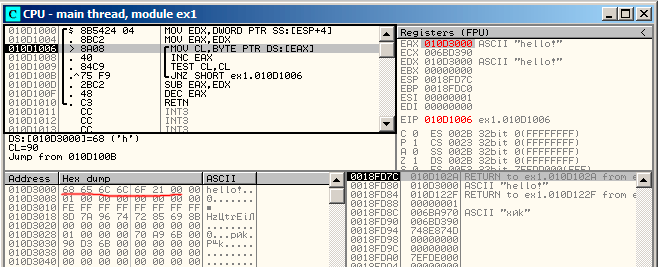
\includegraphics[scale=\FigScale]{patterns/10_strlen/olly1.png}
\caption{\olly: \RU{начало первой итерации}\EN{first iteration begin}}
\label{fig:strlen_olly_1}
\end{figure}

\begin{figure}[H]
\centering
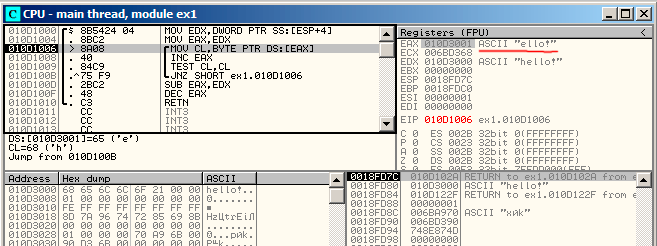
\includegraphics[scale=\FigScale]{patterns/10_strlen/olly2.png}
\caption{\olly: \RU{начало второй итерации}\EN{second iteration begin}}
\label{fig:strlen_olly_2}
\end{figure}

\begin{figure}[H]
\centering
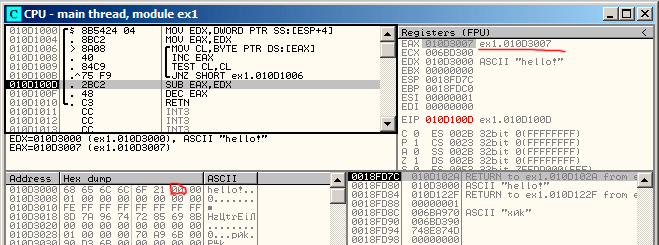
\includegraphics[scale=\FigScale]{patterns/10_strlen/olly3.png}
\caption{\olly: \RU{сейчас будет вычисление разницы указателей}\EN{pointers difference to be calculated now}}
\label{fig:strlen_olly_3}
\end{figure}

\begin{figure}[H]
\centering
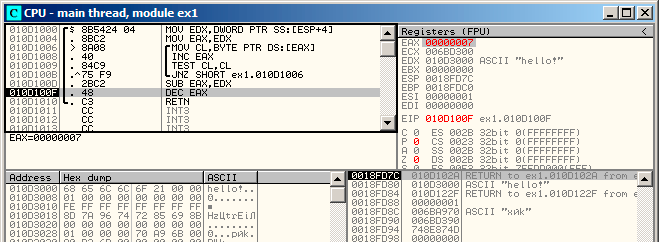
\includegraphics[scale=\FigScale]{patterns/10_strlen/olly4.png}
\caption{\olly: \RU{сейчас будет декремент \EAX}\EN{\EAX to be decremented now}}
\label{fig:strlen_olly_4}
\end{figure}

\subsection{\Optimizing GCC}

\RU{Попробуем GCC 4.4.1 с включенной оптимизацией (ключ \Othree:}
\EN{Let's check GCC 4.4.1 with optimization turned on (\Othree key):}

\lstinputlisting{patterns/10_strlen/10_3_gcc_O3.asm}

\RU{Здесь GCC не очень отстает от MSVC за исключением наличия \MOVZX.} 
\EN{Here GCC is almost the same as MSVC, except of \MOVZX presence.}

\RU{Впрочем, \MOVZX здесь явно можно заменить на}
\EN{However, \MOVZX could be replaced here to} \TT{mov dl, byte ptr [eax]}.

\RU{Но, возможно, компилятору GCC просто проще помнить, что у него под переменную типа \Tchar отведен целый 
32-битный регистр и быть уверенным в том, что старшие биты регистра не будут замусорены.}
\EN{Probably, it is simpler for GCC compiler's code generator to \IT{remember} the whole register 
is allocated for \Tchar variable and it can be sure the highest bits will not contain any noise 
at any point.}

\label{strlen_NOT_ADD}
\index{x86!\Instructions!NOT}
\index{x86!\Instructions!XOR}
\RU{Далее мы видим новую для нас инструкцию \NOT. Эта инструкция инвертирует все биты в операнде. 
Можно сказать, что здесь это синонимично инструкции \TT{XOR ECX, 0ffffffffh}. 
\NOT и следующая за ней инструкция \ADD вычисляют разницу указателей и отнимают от результата единицу. 
Только происходит это слегка по-другому. Сначала \ECX, где хранится указатель на \IT{str}, 
инвертируется и от него отнимается единица.}
\EN{After, we also see new instruction \NOT. This instruction inverts all bits in operand. 
It can be said, it is synonym to the \TT{XOR ECX, 0ffffffffh} instruction. 
\NOT and following \ADD calculating pointer difference and subtracting 1. 
At the beginning \ECX, where pointer to \IT{str} is stored, inverted and 1 is subtracted from it.}

\RU{См. также раздел:}\EN{See also:} ``\SignedNumbersSectionName''~(\ref{sec:signednumbers}).

\RU{Иными словами, в конце функции, после цикла, происходит примерно следующее:} 
\EN{In other words, at the end of function, just after loop body, these operations are executed:}

\begin{lstlisting}
ecx=str;
eax=eos;
ecx=(-ecx)-1; 
eax=eax+ecx
return eax
\end{lstlisting}

\dots \RU{что эквивалентно}\EN{and this is effectively equivalent to}:

\begin{lstlisting}
ecx=str;
eax=eos;
eax=eax-ecx;
eax=eax-1;
return eax
\end{lstlisting}

\RU{Но почему GCC решил, что так будет лучше? Снова не берусь сказать. Но я не сомневаюсь, 
что эти оба варианта работают примерно равноценно в плане эффективности и скорости.}
\EN{Why GCC decided it would be better? I cannot be sure. 
But I'm sure the both variants are effectively equivalent in efficiency sense.}
